\section{Variational Autoencoder}
\label{sec:vae}

Variational Autoencoder (VAE) \cite{vae} is a generative model used to learn the underlying distribution of data and generate new samples (similar to the dataset). The model consists of 3 main components: an \textbf{encoder}, \textbf{latent space} (sometimes called 'code vectors' or 'bottleneck layer') and a \textbf{decoder}. The main idea behind VAE is to use the autoencoder model \cite{autoencoder} \cite{autoencoder2} (figure \ref{figure:autoencoder_architecture}) to compress large dimensional space (in our case, images) into smaller, lower dimension vectors that represent the underlying hidden features. These code vectors are then fed into a decoder network which reconstructs the image (maps latent vectors to high-dimensional space).

Compared to the AE, VAEs gives significant control over how we want to model our latent distribution, which in turn gives \textbf{precise control over the output samples} (see figure \ref{fig:vae_control_latent_space}). This kind of control doesn't exist in the usual autoencoder framework.


\begin{figure}[h]
    \centering
    \begin{tikzpicture}
        % Center point of encoder
        \coordinate (E_CENTER) at (1, 1);
        \coordinate (INPUT_TEXT) at (-0.25, 0.5);



        % Draw input vector
        \draw ($(INPUT_TEXT) + (-0.25, -0.5)$) rectangle ($(INPUT_TEXT) + (0.25, 1.5)$) node[pos=.5] {$x$};
        \draw[->] ($(E_CENTER) + (-1, 0)$) -- (E_CENTER);

        








        % Draw the encoder
        \node at ($(E_CENTER) + (1, 1.5)$) {Encoder};
        
        \coordinate (A) at ($(E_CENTER) + (0, -1)$);
        \coordinate (B) at ($(E_CENTER) + (2, -0.5)$);
        \coordinate (C) at ($(E_CENTER) + (2, 0.5)$);
        \coordinate (D) at ($(E_CENTER) + (0, 1)$);
        \draw[fill=gray!30] (A) -- (B) -- (C) -- (D) -- cycle;
        
        % Define the coordinates for the first set of circles (3 neurons)
        \coordinate (n1) at ($(E_CENTER) + (0.5, -0.5)$);
        \coordinate (n2) at ($(E_CENTER) + (0.5, 0)$);
        \coordinate (n3) at ($(E_CENTER) + (0.5, 0.5)$);
        
        % Define the coordinates for the second set of circles (2 neurons)
        \coordinate (m1) at ($(E_CENTER) + (1.5, 0.25)$);
        \coordinate (m2) at ($(E_CENTER) + (1.5, -0.25)$);
        
        % Draw the first set of circles
        \foreach \i in {n1, n2, n3} {
            \filldraw[fill=white] (\i) circle (6pt);
        }
        
        % Draw the second set of circles
        \foreach \i in {m1, m2} {
            \filldraw[fill=white] (\i) circle (6pt);
        }
        
        % Draw arrows from each circle in the first set to each circle in the second set
        \foreach \i in {n1, n2, n3} {
            \foreach \j in {m1, m2} {
                \draw[-] (\i) -- (\j);
            }
        }






        % Draw code vector

        % Arrow in
        \coordinate (Z_TEXT) at ($(E_CENTER) + (3, 0)$);
        \draw[->] ($(E_CENTER) + (2, 0)$) -- ($(Z_TEXT) + (-0.25, 0)$);

        \draw ($(Z_TEXT) + (-0.25, -0.5)$) rectangle ($(Z_TEXT) + (0.25, 0.5)$) node[pos=.5] {$z$};
        
        % Arrow out
        \coordinate (D_CENTER) at ($(E_CENTER) + (4, 0)$);
        \draw[->] ($(Z_TEXT) + (0.25, 0)$) -- (D_CENTER);











        % Draw decoder
        \node at ($(D_CENTER) + (1, 1.5)$) {Decoder};
        
        \coordinate (A2) at ($(D_CENTER) + (0, 0.5)$);
        \coordinate (B2) at ($(D_CENTER) + (2, 1)$);
        \coordinate (C2) at ($(D_CENTER) + (2, -1)$);
        \coordinate (D2) at ($(D_CENTER) + (0, -0.5)$);
        \draw[fill=gray!30] (A2) -- (B2) -- (C2) -- (D2) -- cycle;
        
        % Define the coordinates for the first set of circles (2 neurons)
        \coordinate (n2_1) at ($(D_CENTER) + (0.5, 0.25)$);
        \coordinate (n2_2) at ($(D_CENTER) + (0.5, -0.25)$);
        
        % Define the coordinates for the second set of circles (3 neurons)
        % \coordinate (m2_1) at (1.5, 0.5);
        % \coordinate (m2_2) at (1.5, 1);
        % \coordinate (m2_3) at (1.5, 1.5);
        \coordinate (m2_1) at ($(n2_1) + (1, 0.25)$);
        \coordinate (m2_2) at ($(n2_1) + (1, -0.25)$);
        \coordinate (m2_3) at ($(n2_1) + (1, -0.75)$);
        
        % Draw the first set of circles
        \foreach \i in {n2_1, n2_2} {
            \filldraw[fill=white] (\i) circle (6pt);
        }
        
        % Draw the second set of circles
        \foreach \i in {m2_1, m2_2, m2_3} {
            \filldraw[fill=white] (\i) circle (6pt);
        }
        
        % Draw arrows from each circle in the first set to each circle in the second set
        \foreach \i in {n2_1, n2_2} {
            \foreach \j in {m2_1, m2_2, m2_3} {
                \draw[-] (\i) -- (\j);
            }
        }


        \coordinate (D_END) at ($(D_CENTER) + (2, 0)$);




        % Draw output vector
        \coordinate (X_OUT_TEXT) at ($(m2_2) + (2, 0)$);
        \draw[->] (D_END) -- ($(X_OUT_TEXT) + (-0.25, 0)$);
        
        \draw ($(X_OUT_TEXT) + (-0.25, -1)$) rectangle ($(X_OUT_TEXT) + (0.25, 1)$) node[pos=.5] {$\hat{x}$};
        
        % \node at (X_OUT_TEXT) {$\hat{x}$};
        
    \end{tikzpicture}
    \caption{Autoencoder architecture.}
\end{figure}


\begin{figure}
    \centering
    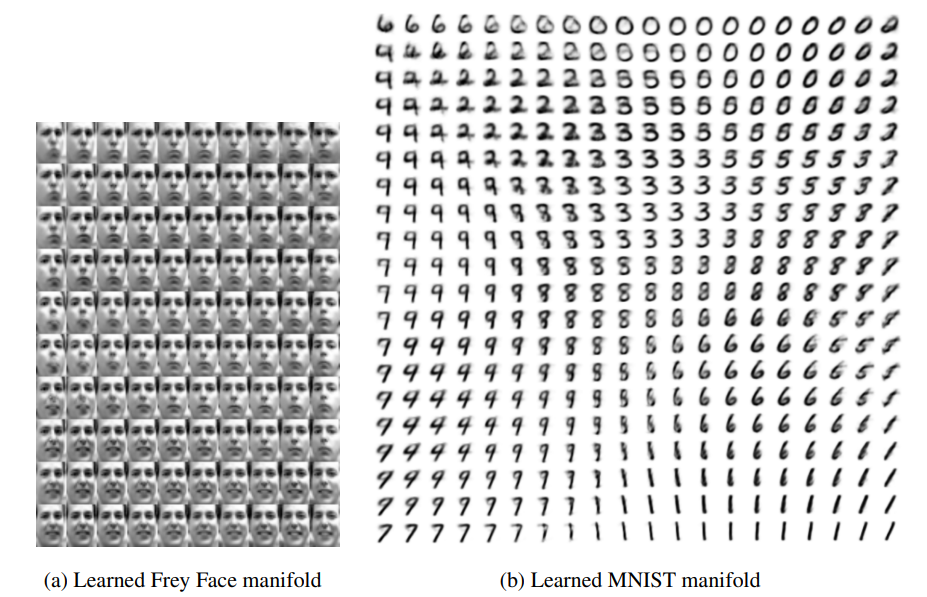
\includegraphics[scale=0.5]{images/vae.png}
    \caption{Visualization a VAE modeled 2D latent space of learned data \cite{vae}, learned on two different datasets. The variational aspect makes it possible to control the generated output. \href{https://ar5iv.labs.arxiv.org/html/1804.00140}{Source}.}
    \label{fig:vae_control_latent_space}
\end{figure}

More formally, the encoder network takes an input data point $x$ and maps it to a latent space representation $z$, which is a compressed representation of $x$. The input is a vector, therefor an image must be flattened from 2D to 1D vector. This flattening will become an issue later in image generation, as this action removes important spatial information and hidden structures in the image. Because of this, modifications were made to the VAE model which allows the capture of spatial information by using a CNN (Convolutional Neural Network) \cite{cnn} layers \cite{vae_cnn_example}, max pooling layers, and other different types of spatial layers. After compression, the latent vector $z$ is then passed onto the decoder for reconstruction. 

The reconstruction is learned by a reconstruction loss function, usually \textbf{mean squared error (MSE)} loss function:

\begin{equation}
    \text{MSE} = \frac{1}{N} \sum_{i=1}^{N} (y_i - \hat{y}_i)^2
\label{eq:mse}
\end{equation}

This loss is used to ensure that the generated images closely resemble the original input images by comparing the \textbf{distance between pixels}, which motivates the model to reconstruct the image to resemble the input image.

During training, both the encoder and decoder are learned with backpropagation, but during inference, only the decoder is used.

The code vectors learned by AE are \textbf{deterministic mapping} from input to code vectors; e.g. the code vectors of images of cats are scattered throughout the entire latent space, whereas in VAE, they are clustered together. 

The latent space in AEs is irregular and discontinuous which makes \textbf{interpolation in the latent space} difficult. VAE solves this problem: it regularizes the latent space by enforcing a prior distribution. This regularization leads to a smooth and continuous latent space (see figure \ref{fig:ae_vs_vae}), which allows the model to interpolate between the latent space smoothly, thus creating similar new images with different variations. In other words, VAE is \textbf{probabilistic model instead of discrete mapper}, like AE.

\begin{figure}[h]
    \centering
    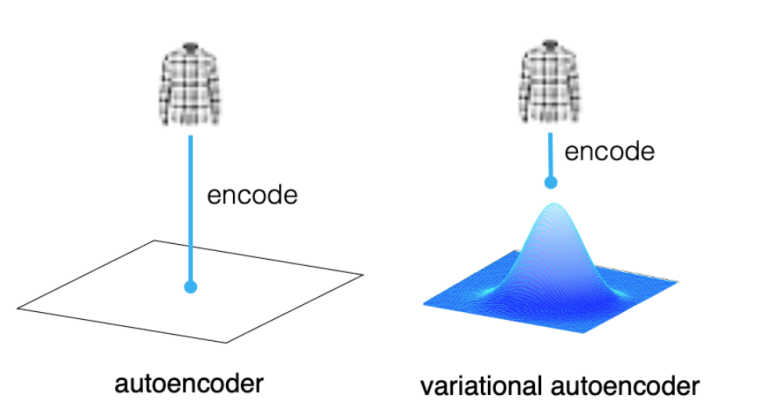
\includegraphics[scale=0.4]{images/autoencoder-vs-variational-autoencoder-point-vs-distribution-768x409.png}
    \caption{Mapping an input image to code vector (left) in AE and mapping an input image to a distribution (right) in VAE \cite{ae_vs_vae}. \href{https://vitalflux.com/autoencoder-vs-variational-autoencoder-vae-difference/}{Source}.}
    \label{fig:ae_vs_vae}
\end{figure}

At the heart of VAE lies the concept of \textbf{latent variables}. Latent variables are hidden, unobserved variables that the model infers from the observed data (dataset). Latent variable models, such as VAE, take indirect approach to describing a probability distribution $p(x)$ over multidimensional variable $x$. Instead of directly writing the expression for $p(x)$, they model a joint distribution $p(x|z)$ of the data $x$ and an unobserved hidden latent variable $z$.

The variational aspect of VAE refers to the use of \textbf{variational inference (VI)}, which is used to approximate complex posterior distributions by transforming the problem into optimization problem:

\begin{equation}
p(z|x) = \frac{p(x|z) \cdot p(z)}{\int p(x|z) \cdot p(z) dz}
\label{eq:vae_posterior}
\end{equation}

The denominator in eq. \ref{eq:vae_posterior} is \textbf{intractable} because it involves integrating over all possible values of $z$, and $z$ is often relatively high-dimensional, and it's infeasible to evaluate exactly. Which is why VI is used, which approximates the true posterior distribution $p(z|x)$ with simpler, tractable distribution $q_\phi (z|x)$, parameterized by $\phi$.

\textbf{Inference}: to generate an image, first we sample a latent variable $z$ from prior distribution $p(z)$, which is typically standard normal distribution $\mathcal{N}(0, 1)$. Then $z$ is passed to the decoder and image $x$ is generated from the conditional distribution $p_\theta (x|z)$. 





\subsection{The Reparameterization Trick}

To enable backpropagation through the sampling process, VAEs use the reparameterization trick. This trick involves expressing the sampled latent variables $z$ as a deterministic function of the encoder's output and some random noise. \textbf{Without this technique, backpropagation would not be possible}, because sampling from a distribution is a stochastic process (involves randomness) and is a non-differentiable operation and the gradients can't be computed with respect to the parameters of the encoder. 

To make the sampling operation differentiable and thus allow gradients to flow through the network, the reparameterization trick is used. Specifically, if $\mu$ and $\sigma$ are the mean and standard deviation vectors outputted by the encoder, we can write:

\begin{equation*}
    z = \mu + \sigma \cdot \epsilon
\end{equation*}

where $\epsilon \sim \mathcal{N}(0, 1)$ is a standard normal random variable. This $\epsilon$ \textbf{will not change throughout the training regime}: it's sampled once and fixed in place.


\begin{figure}[h]
    \centering
    \begin{tikzpicture}
        % Center point of encoder
        \coordinate (E_CENTER) at (1, 1);
        \coordinate (INPUT_TEXT) at (-0.25, 0.5);



        % Draw input vector
        \draw ($(INPUT_TEXT) + (-0.25, -0.5)$) rectangle ($(INPUT_TEXT) + (0.25, 1.5)$) node[pos=.5] {$x$};
        \draw[->] ($(E_CENTER) + (-1, 0)$) -- (E_CENTER);

        








        % Draw the encoder
        \node at ($(E_CENTER) + (1, 1.5)$) {Encoder $q_\phi(z|x)$};
        
        \coordinate (A) at ($(E_CENTER) + (0, -1)$);
        \coordinate (B) at ($(E_CENTER) + (2, -0.5)$);
        \coordinate (C) at ($(E_CENTER) + (2, 0.5)$);
        \coordinate (D) at ($(E_CENTER) + (0, 1)$);
        \draw[fill=gray!30] (A) -- (B) -- (C) -- (D) -- cycle;
        
        % Define the coordinates for the first set of circles (3 neurons)
        \coordinate (n1) at ($(E_CENTER) + (0.5, -0.5)$);
        \coordinate (n2) at ($(E_CENTER) + (0.5, 0)$);
        \coordinate (n3) at ($(E_CENTER) + (0.5, 0.5)$);
        
        % Define the coordinates for the second set of circles (2 neurons)
        \coordinate (m1) at ($(E_CENTER) + (1.5, 0.25)$);
        \coordinate (m2) at ($(E_CENTER) + (1.5, -0.25)$);
        
        % Draw the first set of circles
        \foreach \i in {n1, n2, n3} {
            \filldraw[fill=white] (\i) circle (6pt);
        }
        
        % Draw the second set of circles
        \foreach \i in {m1, m2} {
            \filldraw[fill=white] (\i) circle (6pt);
        }
        
        % Draw arrows from each circle in the first set to each circle in the second set
        \foreach \i in {n1, n2, n3} {
            \foreach \j in {m1, m2} {
                \draw[-] (\i) -- (\j);
            }
        }






        % Draw middle
        \coordinate (Z_TEXT) at ($(E_CENTER) + (3, 0)$);

        \coordinate (MIDDLE_BEGIN) at ($(Z_TEXT) + (-0.5, 0)$);
        \coordinate (MU_BEGIN) at ($(MIDDLE_BEGIN) + (0.25, 0.5)$);
        \coordinate (SIGMA_BEGIN) at ($(MIDDLE_BEGIN) + (0.25, -0.5)$);
        \coordinate (Z_BEGIN) at ($(Z_TEXT) + (0.75, 0)$);

        \coordinate (ARROW_OUT_BEGIN) at ($(Z_TEXT) + (1.75, 0)$);
        \coordinate (ARROW_OUT_END) at ($(ARROW_OUT_BEGIN) + (0.5, 0)$);

        % Middle nodes
        \node[draw,rectangle] (SIGMA) at ($(SIGMA_BEGIN) + (0.5, 0)$) {$\sigma$};
        \node[draw,rectangle] (MU) at ($(MU_BEGIN) + (0.5, 0)$) {$\mu$};
        \node[draw,rectangle] (Z) at ($(Z_BEGIN) + (0.5, 0)$) {$z$};

        % Rectangle around all nodes
        \node[draw, rectangle, inner sep=5pt, fit=(SIGMA) (MU) (Z)] (middle_rect) {};

        % Equations below the rectangle
        \node[below=0cm of middle_rect] (eq1) {$z = \mu + \sigma \cdot \epsilon$};
        \node[below=0cm of eq1] (eq2) {$z \sim \mathcal{N}(\mu, \sigma^2)$};

        % Arrow from trapazoid to rectangle
        \draw[->] ($(E_CENTER) + (2, 0)$) -- (middle_rect);

        % Inner arrows
        \draw[->, to path={-| (\tikztotarget)}] (SIGMA) edge (Z) (MU) edge (Z);











        % Draw decoder
        \coordinate (D_CENTER) at ($(Z_TEXT) + (2.5, 0)$);
        \node at ($(D_CENTER) + (1, 1.5)$) {Decoder $p_\theta(x|z)$};

        % Arrow from the rectangle to the trapezoid
        \draw[->] (middle_rect.east) -- (D_CENTER);

        % Draw trapazoid
        \coordinate (A2) at ($(D_CENTER) + (0, 0.5)$);
        \coordinate (B2) at ($(D_CENTER) + (2, 1)$);
        \coordinate (C2) at ($(D_CENTER) + (2, -1)$);
        \coordinate (D2) at ($(D_CENTER) + (0, -0.5)$);
        \draw[fill=gray!30] (A2) -- (B2) -- (C2) -- (D2) -- cycle;
        
        % Define the coordinates for the first set of circles (2 neurons)
        \coordinate (n2_1) at ($(D_CENTER) + (0.5, 0.25)$);
        \coordinate (n2_2) at ($(D_CENTER) + (0.5, -0.25)$);
        
        % Define the coordinates for the second set of circles (3 neurons)
        \coordinate (m2_1) at ($(n2_1) + (1, 0.25)$);
        \coordinate (m2_2) at ($(n2_1) + (1, -0.25)$);
        \coordinate (m2_3) at ($(n2_1) + (1, -0.75)$);
        
        % Draw the first set of circles
        \foreach \i in {n2_1, n2_2} {
            \filldraw[fill=white] (\i) circle (6pt);
        }
        
        % Draw the second set of circles
        \foreach \i in {m2_1, m2_2, m2_3} {
            \filldraw[fill=white] (\i) circle (6pt);
        }
        
        % Draw arrows from each circle in the first set to each circle in the second set
        \foreach \i in {n2_1, n2_2} {
            \foreach \j in {m2_1, m2_2, m2_3} {
                \draw[-] (\i) -- (\j);
            }
        }


        \coordinate (D_END) at ($(D_CENTER) + (2, 0)$);

        % Draw output vector
        \coordinate (X_OUT_TEXT) at ($(m2_2) + (2, 0)$);
        \draw[->] (D_END) -- ($(X_OUT_TEXT) + (-0.25, 0)$);
        
        \draw ($(X_OUT_TEXT) + (-0.25, -1)$) rectangle ($(X_OUT_TEXT) + (0.25, 1)$) node[pos=.5] {$\hat{x}$};
        
        % \node at (X_OUT_TEXT) {$\hat{x}$};
        
    \end{tikzpicture}
    \caption{Variational Autoencoder architecture.}
    \label{figure:vae}
\end{figure}


The VAE architecture is shown in figure \ref{figure:vae}.

\subsection{Training}

The VAE optimizes the \textbf{Evidence Lower Bound (ELBO)} to ensure that the approximate posterior $q_\phi (z|x)$ is close to the true posterior $p(z|x)$ (we want to maximize it):

\begin{equation}
    \mathcal{L}(\theta, \phi; x, z) = \text{ELBO} = \mathbb{E}_{q_\phi(z|x)} \left[ \log p_\theta(x|z) \right] - D_\text{KL}(q_\phi(z|x) \| p(z))
    \label{eq:vae_elbo}
\end{equation}

where the first term is the \textbf{reconstruction loss} and the second term is the \textbf{KL divergence loss} (which measure how much the approximate posterior $q_\phi (z|x)$ diverges from the prior $p(z)$). 
